\documentclass[fontscale=0.38]{baposter}

\tracingstats=2

\usepackage{times}
\usepackage{calc}
\usepackage{graphicx}
\usepackage{amsmath}
\usepackage{amssymb}
\usepackage{relsize}
\usepackage{multirow}
\usepackage{bm}
\usepackage{caption}
\usepackage[authoryear,round]{natbib}

\usepackage{tabularx}
\usepackage{booktabs}

\usepackage{colortbl}

\usepackage{multicol}

%\usepackage{pgfbaselayers}
%\pgfdeclarelayer{background}
%\pgfdeclarelayer{foreground}
%\pgfsetlayers{background,main,foreground}


% plr macros: these are for boxes in tables
\newcommand\tLL[1]{\multicolumn{1}{|c}{#1}}
\newcommand\tRR[1]{\multicolumn{1}{c|}{#1}}
\newcommand\tLR[1]{\multicolumn{1}{|c|}{#1}}
% nucleotides:
\newcommand{\nA}{\mbox{A}}  
\newcommand{\nC}{\mbox{C}}
\newcommand{\nG}{\mbox{G}}
\newcommand{\nT}{\mbox{T}}


%\usepackage{tikz}
%\usetikzlibrary{arrows,backgrounds,patterns,matrix,shapes,fit,calc,shadows,plotmarks,decorations.pathmorphing,positioning,trees}

\renewcommand{\familydefault}{\sfdefault}
\usepackage{helvet}
\usepackage{bookman}
\usepackage{palatino}

% My stuff
\newcommand{\E}{\mathbb{E}}
\renewcommand{\P}{\mathbb{P}}
% end my stuff

\selectcolormodel{cmyk}

% \graphicspath{{images/}}

%%%%%%%%%%%%%%%%%%%%%%%%%%%%%%%%%%%%%%%%%%%%%%%%%%%%%%%%%%%%%%%%%%%%%%%%%%%%%%%%
%%%% Some symbols used in the text
%%%%%%%%%%%%%%%%%%%%%%%%%%%%%%%%%%%%%%%%%%%%%%%%%%%%%%%%%%%%%%%%%%%%%%%%%%%%%%%%
%\newcommand{\sub}[2]{\ensuremath{#1_{\textrm{#2}}}}
%\newcommand{\gen}[2]{\ensuremath{\textrm{#1}_{\textrm{#2}}}}


%%%%%%%%%%%%%%%%%%%%%%%%%%%%%%%%%%%%%%%%%%%%%%%%%%%%%%%%%%%%%%%%%%%%%%%%%%%%%%%%
% Multicol Settings
%%%%%%%%%%%%%%%%%%%%%%%%%%%%%%%%%%%%%%%%%%%%%%%%%%%%%%%%%%%%%%%%%%%%%%%%%%%%%%%%
%\setlength{\columnsep}{0.7em}
\setlength{\columnsep}{8mm}
\setlength{\columnseprule}{0mm} % no vertical line


%%%%%%%%%%%%%%%%%%%%%%%%%%%%%%%%%%%%%%%%%%%%%%%%%%%%%%%%%%%%%%%%%%%%%%%%%%%%%%%%
% Save space in lists. Use this after the opening of the list
%%%%%%%%%%%%%%%%%%%%%%%%%%%%%%%%%%%%%%%%%%%%%%%%%%%%%%%%%%%%%%%%%%%%%%%%%%%%%%%%
\newcommand{\compresslist}{
\setlength{\itemsep}{1pt}
\setlength{\parskip}{0pt}
\setlength{\parsep}{0pt}
}

%%%%%%%%%%%%%%%%%%%%%%%%%%%%%%%%%%%%%%%%%%%%%%%%%%%%%%%%%%%%%%%%%%%%%%%%%%%%%%
%%% Other Macros
%%%%%%%%%%%%%%%%%%%%%%%%%%%%%%%%%%%%%%%%%%%%%%%%%%%%%%%%%%%%%%%%%%%%%%%%%%%%%%
% \renewcommand{\labelenumi}{\alph{enumi})}
% \renewcommand{\theenumi}{\alph{enumi})}
\newcommand{\postercaption}[1]{\begin{minipage}{\linewidth}\center\smaller
  {#1}\end{minipage}}



%%%%%%%%%%%%%%%%%%%%%%%%%%%%%%%%%%%%%%%%%%%%%%%%%%%%%%%%%%%%%%%%%%%%%%%%%%%%%%
%%% Begin of Document
%%%%%%%%%%%%%%%%%%%%%%%%%%%%%%%%%%%%%%%%%%%%%%%%%%%%%%%%%%%%%%%%%%%%%%%%%%%%%%

\begin{document}

%%%%%%%%%%%%%%%%%%%%%%%%%%%%%%%%%%%%%%%%%%%%%%%%%%%%%%%%%%%%%%%%%%%%%%%%%%%%%%
%%% Here starts the poster
%%%---------------------------------------------------------------------------
%%% Format it to your taste with the options
%%%%%%%%%%%%%%%%%%%%%%%%%%%%%%%%%%%%%%%%%%%%%%%%%%%%%%%%%%%%%%%%%%%%%%%%%%%%%%

% Define some colors
\definecolor{silver}{cmyk}{0,0,0,0.3}
\definecolor{black}{cmyk}{0,0,0.0,1.0}
\definecolor{white}{cmyk}{0,0,0.0,0.0}
\definecolor{darkSilver}{cmyk}{0,0,0,0.1}

\definecolor{darkYellow}{cmyk}{0,0,1.0,0.5}
\definecolor{yellow}{cmyk}{0,0,0.9,0.0}
\definecolor{reddishyellow}{cmyk}{0,0.22,1.0,0.0}
\definecolor{lightyellow}{cmyk}{0,0,0.3,0.0}
\definecolor{lighteryellow}{cmyk}{0,0,0.1,0.0}
\definecolor{lightestyellow}{cmyk}{0,0,0.05,0.0}

\definecolor{DavisBlue}{cmyk}{1,0.56,0,0.34}
%    C = 100  M = 56  Y = 0 K = 34


\definecolor{HohenheimBlue}{cmyk}{1,0.5,0,0.45}
\definecolor{HohenheimLightLightBlue}{RGB}{243,250,255}
\definecolor{HohenheimLightBlue}{RGB}{215,221,235}
\definecolor{HohenheimDarkBlue}{RGB}{52,104,152}
\definecolor{darkCyan}{cmyk}{1,1,0,0.5}
\definecolor{cyan}{cmyk}{1,0,0,0.0}
\definecolor{lightcyan}{cmyk}{0.3,0,0,0.0}
\definecolor{lightercyan}{cmyk}{0.1,0,0,0.0}
\definecolor{lightestcyan}{cmyk}{0.05,0,0,0.0}



\typeout{Poster Starts}
%Define custom background
\background{
  \begin{tikzpicture}[remember picture,overlay]%
    \draw (current page.north west)+(-2em,2em) node[anchor=north west] {\includegraphics[height=\textheight]{silhouettes_background}};
  \end{tikzpicture}%
}

\newlength{\leftimgwidth}
\begin{poster}%
  % Poster Options
  {
  % Columns and Column spacing
  columns=2,
  colspacing=1.5em,
  % Background
  % background=user,
  background=shade-tb,
  % Poster header options
  eyecatcher=yes,
  posterheaderheight=0.15\textheight,
  % Format of textbox header
  headerborder=open,
  % headershape=small-rounded,
  headershape=roundedright,
  headershade=shade-tb,
  % headershade=plain,
  headerfont=\Large\textsf, %Sans Serif
  % Format of textbox
  boxborder=small-rounded,
  % boxborder=roundedleft,    
  boxshade=plain,
  linewidth=0.5pt,
  % Color style
  % bgColorOne=lightestcyan,
  % bgColorTwo=lightcyan,
  bgColorOne=white,
  bgColorTwo=white,
  % borderColor=cyan,
  borderColor=black,
  headerColorOne=DavisBlue,
  % headerColorOne=cyan,
  headerColorTwo=black,
  % headerFontColor=black,
  headerFontColor=white,
  % boxColorOne=lightercyan,
  boxColorOne=HohenheimLightLightBlue,
  boxColorTwo=white,
  % Show grid to help with alignment
  grid=no
  % grid=yes
  }
  % Eye Catcher
  {
  \makebox[15em][r]{%
    \begin{minipage}{15em}
       \hfill
       
\includegraphics[width=15em]{USC-seal} \\
    \end{minipage}
    }
  }
  % Title
  {\sf %Sans Serif
  %\bf% %bold  
  \vspace{0.5em}
  \textbf{\textcolor{DavisBlue}{Efficient inference with context-dependent models of nucleotide substituion}}\vspace{0.5em}}
  % Authors
  {\sf %Sans Serif
    Peter Ralph$^{\dagger}$ \\  \vspace{-1.0mm}
    {\small \textit{$\dagger$ Molecular \& Computational Biology, University of Southern California }}\\  
    {\small   \textbf{ralphlab.usc.edu}}\\
  }
  % Project logo
  {
    \makebox[15em][r]{%
      \begin{minipage}{15em}
        \hfill
        
\includegraphics[width=15em]{../../contextual-logo}
      \end{minipage}
    }
  }

  % Width of left inset image
%  \setlength{\leftimgwidth}{0.78em+0.0em}

%%%%%%%%%%%%%%%%%%%%%%%%%%%%%%%%%%%%%%%%%%%%%%%%%%%%%%%%%%%%%%%%%%%%%%%%%%%%%%
%%% Now define the boxes that make up the poster
%%%---------------------------------------------------------------------------
%%% Each box has a name and can be placed absolutely or relatively.
%%% The only inconvenience is that you can only specify a relative position 
%%% towards an already declared box. So if you have a box attached to the 
%%% bottom, one to the top and a third one which should be in between, you 
%%% have to specify the top and bottom boxes before you specify the middle 
%%% box.
%%%%%%%%%%%%%%%%%%%%%%%%%%%%%%%%%%%%%%%%%%%%%%%%%%%%%%%%%%%%%%%%%%%%%%%%%%%%%%

%%%%%%%%%%%%%%%%%%%%%%%%%%%%%%%%%%%%%%%%%%%%%%%%%%%%%%%%%%%%%%%%%%%%%%%%%%%%%%
\headerbox{Context-dependence}{name=intro,column=0,row=0,span=1}{
%%%%%%%%%%%%%%%%%%%%%%%%%%%%%%%%%%%%%%%%%%%%%%%%%%%%%%%%%%%%%%%%%%%%%%%%%%%%%%

  \textbf{Given} long, homologous sequences with known phylogenetic relationship, \\
  that have mutated from an ancestral sequence by a
  \textbf{context-dependent substitution process},
  \textbf{our goal} is to infer substitution motifs;
    mutation rates; and branch lengths on the tree.

    \vspace{2em}

  \textbf{Background:} 
  The raw mutational spectrum is highly context-dependent % and multinuleotide 
  \citep{schaibley2013influence}. %,schrider2011pervasive,terekhanova2013prevalence,harris2013errorprone}.
  This is an issue for methods in phylogenetics and ancestral sequence reconstruction
  that assume independence of sites.
  Previous  methods --
  \citet{siepel2004phylogenetic} assumed Markov dependency along the sequence;
  \citet{lunter2004nucleotide} used a matrix decomposition;
  and \citet{pedersen2000dependent,hobolth2008markov} used data augmentation with an MCMC algorithm
  -- are not computationally feasible for long sequences.
  Similar problem -- Markov random fields in image reconstruction \citep{besag1986statistical};
  inference for cellular automata models \citep{zorzenondossantos2001dynamics}.

}
%%%%%%%%%%%%%%%%%%%%%%%%%%%%%%%%%%%%%%%%%%%%%%%%%%%%%%%%%%%%%%%%%%%%%%%%%%%%%%


%%%%%%%%%%%%%%%%%%%%%%%%%%%%%%%%%%%%%%%%%%%%%%%%%%%%%%%%%%%%%%%%%%%%%%%%%%%%%%
\headerbox{General mutational grammar}{name=grammar,column=0,span=1,below=intro}{
%%%%%%%%%%%%%%%%%%%%%%%%%%%%%%%%%%%%%%%%%%%%%%%%%%%%%%%%%%%%%%%%%%%%%%%%%%%%%%


    \textbf{Parameters:} an arbitrary set of mutation rules $(a,b,r)$: 
    sequences matching $a$ mutate to $b$ at rate $r$ per unit time;
    $a$ and $b$ can be any patterns of the same length,
    e.g.
    \begin{align*}
        \nA &\longrightarrow \nT \qquad \text{ at rate } 10^{-8} , \\
        \text{or} \qquad       \nC\nA\nC &\longrightarrow \nC\nT\nC \qquad \text{ at rate } 5\times 10^{-8} .
  \end{align*}

%   \textbf{Fixation} function: 
%     mutations take effect with probability 
%     \begin{align*}
%       f(s(\text{new}) - s(\text{old})) ,
%     \end{align*}
%     e.g.\ $f(ds) = N_e (1-e^{-2 ds})/(1-e^{-2 N_e ds})$
% 
%   \textbf{Selection} is additive (and abstract):
%     given rules $(a_i,s_i)$,
%     \begin{align*}
%       s(x) = \sum_i s_i n_i(x),
%     \end{align*}
%     with $n_i(x)$ number of times $a_i$ matches in $x$


    \vspace{1em}

    \textbf{Assuming:}
    homogeneity along the sequence and along each branch; no indels
    \vspace{.5em}

    \textbf{Not assuming:}
    stationarity;
    reversibility.
    (\textbf{e.g.} GC-content need not be at equilibrium)

    % \hrule{\hfill}


  \parbox[b]{.4\textwidth}{

    \textbf{Simple example} on two nucleotides:
      \begin{itemize}
        \item $\text{X} \to \text{O}$ at rate 1
        \item $\text{O} \to \text{X}$ at rate 1
        \item $\text{OX} \to \text{XO}$ at rate $\gamma$
      \end{itemize}
      From before/after sequence, infer $\gamma$.

  }\parbox[b]{.3\textwidth}{

    % easy
    \begin{center} \tiny \setlength{\tabcolsep}{0pt} \begin{tabular}{cccccccccccccccccccccccccccccccccccccccccc}
        \multicolumn{20}{ c }{\textbf{easy:}} \\
    O&O&O&X&O&X&X&X&X&X&X&O&O&O&X&O&X&O&X&O\\
    $\centerdot$&$\centerdot$&$\centerdot$&$\centerdot$&$\centerdot$&$\centerdot$&$\centerdot$&$\centerdot$&$\centerdot$&$\centerdot$&$\centerdot$&$\centerdot$&$\centerdot$&$\centerdot$&$\centerdot$&$\centerdot$&$\centerdot$&$\centerdot$&$\centerdot$&$\centerdot$\\
    $\centerdot$&$\centerdot$&$\centerdot$&$\centerdot$&$\centerdot$&$\centerdot$&$\centerdot$&$\centerdot$&$\centerdot$&$\centerdot$&$\centerdot$&X&$\centerdot$&$\centerdot$&$\centerdot$&$\centerdot$&$\centerdot$&$\centerdot$&$\centerdot$&$\centerdot$\\
    $\centerdot$&$\centerdot$&$\centerdot$&$\centerdot$&$\centerdot$&$\centerdot$&$\centerdot$&$\centerdot$&$\centerdot$&$\centerdot$&$\centerdot$&$\centerdot$&$\centerdot$&$\centerdot$&$\centerdot$&$\centerdot$&$\centerdot$&$\centerdot$&O&X\\
    $\centerdot$&$\centerdot$&$\centerdot$&$\centerdot$&$\centerdot$&$\centerdot$&$\centerdot$&$\centerdot$&$\centerdot$&$\centerdot$&$\centerdot$&$\centerdot$&$\centerdot$&$\centerdot$&O&X&$\centerdot$&$\centerdot$&$\centerdot$&$\centerdot$\\
    $\centerdot$&$\centerdot$&$\centerdot$&$\centerdot$&$\centerdot$&$\centerdot$&$\centerdot$&$\centerdot$&$\centerdot$&$\centerdot$&$\centerdot$&$\centerdot$&$\centerdot$&$\centerdot$&$\centerdot$&$\centerdot$&$\centerdot$&$\centerdot$&$\centerdot$&$\centerdot$\\
    $\centerdot$&$\centerdot$&$\centerdot$&$\centerdot$&$\centerdot$&O&$\centerdot$&$\centerdot$&$\centerdot$&$\centerdot$&$\centerdot$&$\centerdot$&$\centerdot$&$\centerdot$&$\centerdot$&$\centerdot$&$\centerdot$&X&O&$\centerdot$\\
    $\centerdot$&$\centerdot$&$\centerdot$&$\centerdot$&$\centerdot$&$\centerdot$&$\centerdot$&$\centerdot$&$\centerdot$&$\centerdot$&$\centerdot$&$\centerdot$&$\centerdot$&$\centerdot$&$\centerdot$&$\centerdot$&$\centerdot$&$\centerdot$&$\centerdot$&$\centerdot$\\
    $\centerdot$&$\centerdot$&$\centerdot$&$\centerdot$&$\centerdot$&$\centerdot$&$\centerdot$&$\centerdot$&O&$\centerdot$&$\centerdot$&$\centerdot$&$\centerdot$&$\centerdot$&$\centerdot$&$\centerdot$&$\centerdot$&$\centerdot$&$\centerdot$&X\\
    $\centerdot$&$\centerdot$&$\centerdot$&$\centerdot$&$\centerdot$&$\centerdot$&$\centerdot$&$\centerdot$&X&$\centerdot$&$\centerdot$&O&X&$\centerdot$&$\centerdot$&$\centerdot$&$\centerdot$&$\centerdot$&$\centerdot$&$\centerdot$\\
    $\centerdot$&$\centerdot$&$\centerdot$&$\centerdot$&$\centerdot$&$\centerdot$&$\centerdot$&$\centerdot$&$\centerdot$&$\centerdot$&$\centerdot$&$\centerdot$&$\centerdot$&$\centerdot$&$\centerdot$&$\centerdot$&$\centerdot$&$\centerdot$&$\centerdot$&$\centerdot$\\
    O&O&O&X&O&O&X&X&X&X&X&O&X&O&O&X&X&X&X&X\\
    \end{tabular} \end{center} 

  }\parbox[b]{.3\textwidth}{
     
    % hard
    \begin{center} \tiny \setlength{\tabcolsep}{0pt} \begin{tabular}{cccccccccccccccccccccccccccccccccccccccccc}
        \multicolumn{20}{ c }{\textbf{hard:}} \\
    X&O&X&X&O&O&X&X&O&X&O&O&X&O&O&X&O&X&X&O\\
    O&X&O&$\centerdot$&$\centerdot$&$\centerdot$&$\centerdot$&$\centerdot$&$\centerdot$&$\centerdot$&$\centerdot$&$\centerdot$&O&$\centerdot$&$\centerdot$&$\centerdot$&$\centerdot$&$\centerdot$&$\centerdot$&$\centerdot$\\
    $\centerdot$&O&X&$\centerdot$&$\centerdot$&$\centerdot$&O&$\centerdot$&$\centerdot$&$\centerdot$&$\centerdot$&$\centerdot$&$\centerdot$&$\centerdot$&$\centerdot$&$\centerdot$&O&$\centerdot$&$\centerdot$&$\centerdot$\\
    $\centerdot$&X&$\centerdot$&$\centerdot$&$\centerdot$&$\centerdot$&$\centerdot$&$\centerdot$&$\centerdot$&O&$\centerdot$&$\centerdot$&$\centerdot$&$\centerdot$&$\centerdot$&$\centerdot$&$\centerdot$&$\centerdot$&O&$\centerdot$\\
    $\centerdot$&$\centerdot$&$\centerdot$&$\centerdot$&$\centerdot$&$\centerdot$&$\centerdot$&$\centerdot$&X&$\centerdot$&$\centerdot$&$\centerdot$&$\centerdot$&$\centerdot$&$\centerdot$&O&X&$\centerdot$&X&$\centerdot$\\
    $\centerdot$&$\centerdot$&O&$\centerdot$&$\centerdot$&$\centerdot$&$\centerdot$&$\centerdot$&$\centerdot$&$\centerdot$&$\centerdot$&X&$\centerdot$&$\centerdot$&$\centerdot$&$\centerdot$&$\centerdot$&$\centerdot$&$\centerdot$&$\centerdot$\\
    $\centerdot$&$\centerdot$&$\centerdot$&$\centerdot$&$\centerdot$&$\centerdot$&$\centerdot$&$\centerdot$&$\centerdot$&$\centerdot$&$\centerdot$&$\centerdot$&$\centerdot$&$\centerdot$&$\centerdot$&$\centerdot$&$\centerdot$&$\centerdot$&$\centerdot$&$\centerdot$\\
    $\centerdot$&$\centerdot$&$\centerdot$&O&$\centerdot$&$\centerdot$&$\centerdot$&$\centerdot$&$\centerdot$&$\centerdot$&$\centerdot$&$\centerdot$&$\centerdot$&$\centerdot$&$\centerdot$&$\centerdot$&$\centerdot$&$\centerdot$&$\centerdot$&X\\
    $\centerdot$&$\centerdot$&$\centerdot$&$\centerdot$&$\centerdot$&$\centerdot$&$\centerdot$&$\centerdot$&$\centerdot$&$\centerdot$&$\centerdot$&O&$\centerdot$&X&$\centerdot$&$\centerdot$&$\centerdot$&$\centerdot$&$\centerdot$&$\centerdot$\\
    $\centerdot$&$\centerdot$&$\centerdot$&$\centerdot$&$\centerdot$&$\centerdot$&$\centerdot$&$\centerdot$&O&X&$\centerdot$&$\centerdot$&$\centerdot$&$\centerdot$&$\centerdot$&X&$\centerdot$&$\centerdot$&O&$\centerdot$\\
    $\centerdot$&$\centerdot$&$\centerdot$&$\centerdot$&$\centerdot$&X&X&$\centerdot$&$\centerdot$&$\centerdot$&$\centerdot$&$\centerdot$&$\centerdot$&$\centerdot$&$\centerdot$&$\centerdot$&$\centerdot$&$\centerdot$&$\centerdot$&$\centerdot$\\
    O&X&O&O&O&X&X&X&O&X&O&O&O&X&O&X&X&O&O&X\\
    \end{tabular} \end{center} 

  }



}
%%%%%%%%%%%%%%%%%%%%%%%%%%%%%%%%%%%%%%%%%%%%%%%%%%%%%%%%%%%%%%%%%%%%%%%%%%%%%%

%%%%%%%%%%%%%%%%%%%%%%%%%%%%%%%%%%%%%%%%%%%%%%%%%%%%%%%%%%%%%%%%%%%%%%%%%%%%%%
\headerbox{Idea: count \emph{asymmetric} tuples}{name=windows,column=0,span=1,below=grammar}{
%%%%%%%%%%%%%%%%%%%%%%%%%%%%%%%%%%%%%%%%%%%%%%%%%%%%%%%%%%%%%%%%%%%%%%%%%%%%%%

\parbox[b]{.55\textwidth}{

    \begin{itemize}
      \item If the size of the maximum context is $k$
      \item and the mean density of mutations is $\mu t$ per site
      \item \textbf{then} a site is unlikely to be affected by context further away than, say, $k^2 \mu t$.
      \item i.e.\ the sequence at a site, conditioned on a $(k^2 \mu t)$-window in the ancestor,
        is almost independent of the sequence further away.
    \end{itemize}

    }\parbox[b]{.45\textwidth}{

        \vspace{-1em}
    \begin{flushright}
        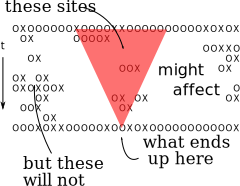
\includegraphics[width=.35\textwidth]{context-illustration}
    \end{flushright}

    }

    \vspace{1em}

    \textbf{Method:}
Count pairs of $(w,r)$-tuples, with $r<w$;
compute exact transition probabilities using $w$-tuples (below);
assume nonoverlapping blocks are independent (binomial likelihood).

\vspace{1em}

\textbf{Example, $(w,r)=(3,1)$:}
  \begin{center} 
    \setlength{\tabcolsep}{0pt} 
    \begin{tabular}{r cccccccccc}
        & $\vert\!\leftarrow$ & $w$ & $\rightarrow\!\vert$ & &&&&&& \\
      \cline{2-4}
      sequence 1 \hspace{2em} & \tLL{C}&C&\tRR{C}&A&G&T&C&C&A&G\\
      \cline{2-2}\cline{4-4}
      sequence 2 \hspace{2em} & C&\tLR{A}&C&A&G&T&C&C&A&G\\
      \cline{3-3}
      & $\rightarrow\!\vert$ & $r$ & $\vert\!\leftarrow$ & &&&&&& \\
    \end{tabular} 
    \hspace{5em}
    \setlength{\tabcolsep}{5pt} 
    \begin{tabular}{c c c}
      $w$-tuple & $r$-tuple & count \\
      \hline
      CCA & C & 2 \\
      CCC & A & 1 \\
      CAG & A & 1 \\
      AGT & G & 1 \\
      \vdots & \vdots & \vdots \\
      \hline
    \end{tabular}
  \end{center} 

  \vspace{1em}

  \textbf{An inference strategy:}
  \begin{itemize}
    \item Fit a simple model with short patterns (e.g.\ $(w,r)=(4,2)$).
    \item Predict longer patterns (e.g.\ $(w,r)=8,4$), and examine residuals.
    \item Add new mutation pattern(s) that best explains residuals.
    \item Repeat until residuals fit the null.
  \end{itemize}

%   \begin{align*}
%     \mathcal{L} = \prod_{a,c} n(a,c) \sum_{b \supset c} \log \left( e^{tG_w} \right)_{ab} .
%   \end{align*}

}
%%%%%%%%%%%%%%%%%%%%%%%%%%%%%%%%%%%%%%%%%%%%%%%%%%%%%%%%%%%%%%%%%%%%%%%%%%%%%%



%%%%%%%%%%%%%%%%%%%%%%%%%%%%%%%%%%%%%%%%%%%%%%%%%%%%%%%%%%%%%%%%%%%%%%%%%%%%%%
\headerbox{Exact solution (for very short sequences)}{name=exact,column=0,span=1,below=windows}{
%%%%%%%%%%%%%%%%%%%%%%%%%%%%%%%%%%%%%%%%%%%%%%%%%%%%%%%%%%%%%%%%%%%%%%%%%%%%%%

Say $\lambda$ is the \emph{total mutation rate}
and $P$ is the matrix of single-mutation probabilities, i.e.
\begin{align}
  \P\{ x \longrightarrow y \text{ in time $dt$ }\} = P_{xy} \lambda dt 
\end{align}
e.g.\ $P_{\scriptsize \nA\nC\nA \to \nA\nT\nA} = \mu_{\scriptsize \nC\nT}$ and $P_{\scriptsize \nG\nA\nC \to \nT\nC\nG} = 0$.
Then the transition probabilities are
\begin{align}
  & \P\{ x \longrightarrow y \text{ in time $t$ }\} = \sum_{k \ge 0} e^{-\lambda t} \frac{ (\lambda t)^k }{ k! } (P^k)_{xy} \\
  &\qquad = \sum_{k \ge 0} \text{( prob there are $k$ mutations )} \times \text{ ( prob k mutations takes $x \to y$ ) } .
\end{align}

$P$ {also equals} $e^{tG}$ with $G_{xy} = \lambda P_{xy}$ and $G_{xx} = - \sum_{y\neq x} G_{xy}$.
Danger: $P$ and $G$ are both $4^w \times 4^w$.

% \[ % max rate < 1 :
% e^{tG}  = e^{t((G+I)-I)} = e^{-t} I e^{t(G+I)} = \sum_k e^{-t} t^k/k! (G+I)^k
% \]
% If $G$ is the \emph{rate matrix}, i.e. for $x \neq y$,
% \begin{align}
%   G_{xy} &= ( \text{ rate at which sequence $x$ changes to $y$ } ) 
% \end{align}
% and $G_{xx} = - \sum_{y\neq x} G_{xy}$, then


}
%%%%%%%%%%%%%%%%%%%%%%%%%%%%%%%%%%%%%%%%%%%%%%%%%%%%%%%%%%%%%%%%%%%%%%%%%%%%%%


%%%%%%%%%%%%%%%%%%%%%%%%%%%%%%%%%%%%%%%%%%%%%%%%%%%%%%%%%%%%%%%%%%%%%%%%%%%%%%
\headerbox{Computation}{name=computation,column=1}{
%%%%%%%%%%%%%%%%%%%%%%%%%%%%%%%%%%%%%%%%%%%%%%%%%%%%%%%%%%%%%%%%%%%%%%%%%%%%%%

\textbf{Speed:} Krylov methods to compute $e^{tG}v$ for sparse $G$;
precompute mapping of parameters to $G$ to make parameter update quick.


  \vspace{1em}

  \textbf{Choices:}
  \begin{itemize}
    \item Long ($w$) and short ($r$) pattern sizes
    \item Set of short patterns, overlapped or not
  \end{itemize}

  \vspace{1em}

  \textbf{Memory usage:} constant times the (pattern count) data.

  \vspace{1em}

  \textbf{Computational time:} $O(w 4^{w} (\#\text{short patterns}))$ operations 
  \begin{itemize}
    \item $(w=5,r=1) \longrightarrow$  a second
    \item $(w=8,r=2) \longrightarrow$  a minute
  \end{itemize}

  \vspace{1em}

  \textbf{Feasible:} window sizes
  \begin{itemize}
    \item  $w=4$: mean density of mutations ${} < 0.5$ per site
    \item  $w=8$: mean density of mutations ${} < 2$ per site
  \end{itemize}


}
%%%%%%%%%%%%%%%%%%%%%%%%%%%%%%%%%%%%%%%%%%%%%%%%%%%%%%%%%%%%%%%%%%%%%%%%%%%%%%


%%%%%%%%%%%%%%%%%%%%%%%%%%%%%%%%%%%%%%%%%%%%%%%%%%%%%%%%%%%%%%%%%%%%%%%%%%%%%%
\headerbox{Simulation: power analysis}{name=simulation,column=1,below=computation}{
%%%%%%%%%%%%%%%%%%%%%%%%%%%%%%%%%%%%%%%%%%%%%%%%%%%%%%%%%%%%%%%%%%%%%%%%%%%%%%


  Simulated $10^6$ bases on a tree of length 1, 
  with one branch twice as long as the other,
  sequence divergence above 15\%;
  estimated single-base + CpG mutation rates, root nucleotide composition, branch asymmetry.
  Priors on the 17 parameters; MCMC to get posterior distribution;
  $w=3$ and $r=1$. Red lines are the truth; boxplots show posterior distribution.

  \begin{center}
    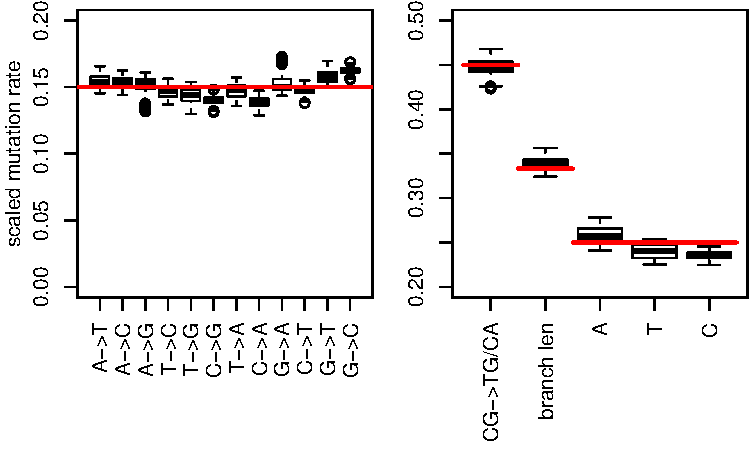
\includegraphics[width=.7\textwidth]{../../../writeup-plots/selsims-2013-06-03-13-17-0187525-estimate-boxplots}
  \end{center}

  

}
%%%%%%%%%%%%%%%%%%%%%%%%%%%%%%%%%%%%%%%%%%%%%%%%%%%%%%%%%%%%%%%%%%%%%%%%%%%%%%


%%%%%%%%%%%%%%%%%%%%%%%%%%%%%%%%%%%%%%%%%%%%%%%%%%%%%%%%%%%%%%%%%%%%%%%%%%%%%%
\headerbox{Real data: mouse--rat noncoding alignment}{name=data,column=1,below=simulation}{
%%%%%%%%%%%%%%%%%%%%%%%%%%%%%%%%%%%%%%%%%%%%%%%%%%%%%%%%%%%%%%%%%%%%%%%%%%%%%%

\textbf{20MB} in 500 noncoding regions in mouse (chosen by Matt Dean), 
aligned to rat (UCSC, mm9--rn5) with gaps and low-quality bases removed,
divergence of 14.7\%.
Fit model with separate single-base mutations + CpG rates,
root nucleotide composition, and branch asymmetry.
using (5,3)--tuples;
looked for structure in residuals of (7,3)--tuples.

\vspace{1em}

\textbf{Preliminary results:} CpG higher than other rates by $10\times{}$;
transitions about $3\times{}$ higher than transversions;
C$\to$A very rare.
Nonstationary CG--content and issue.
Residuals mostly explained by strand slippage.


  \begin{center}
    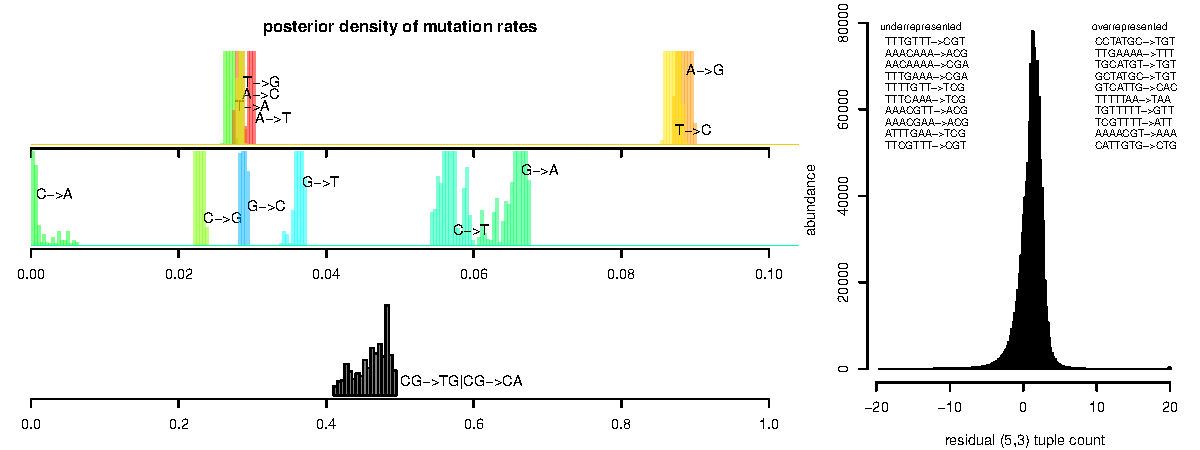
\includegraphics[width=\textwidth]{../../../mus/mm9rn5/poster-results}
  \end{center}


}
%%%%%%%%%%%%%%%%%%%%%%%%%%%%%%%%%%%%%%%%%%%%%%%%%%%%%%%%%%%%%%%%%%%%%%%%%%%%%%

%%%%%%%%%%%%%%%%%%%%%%%%%%%%%%%%%%%%%%%%%%%%%%%%%%%%%%%%%%%%%%%%%%%%%%%%%%%%%%
\headerbox{Summary, and References}{name=references,column=1,above=bottom}{
%%%%%%%%%%%%%%%%%%%%%%%%%%%%%%%%%%%%%%%%%%%%%%%%%%%%%%%%%%%%%%%%%%%%%%%%%%%%%%
    Efficient, provably correct inference and evaluation of model fit
    with arbitrary context-dependent mutation is possible.
    The main limitation is the assumption of homogeneity.
    Other applications: ancestral sequence reconstruction, rigorous hotspot identification\ldots

    \vspace{1em}

    \textbf{Code:} available now/soon at \texttt{http://github.com/petrelharp/context}\\
  \scriptsize
  \renewcommand{\section}[2]{\vskip 0.0em}
  \bibliographystyle{abbrvnat}
  \setlength{\bibsep}{0.0pt}
  \bibliography{context-dependence-poster}
  }
%%%%%%%%%%%%%%%%%%%%%%%%%%%%%%%%%%%%%%%%%%%%%%%%%%%%%%%%%%%%%%%%%%%%%%%%%%%%%%

\end{poster}%
\end{document}
